\documentclass[../Main.tex]{subfiles}
\begin{document}

\section*{Introduction}
\addcontentsline{toc}{section}{Introduction}

Having established the theoretical foundations of single-agent and multi-agent reinforcement learning, this chapter transitions from theory to practice. It details the full lifecycle of our experimental investigation, from the initial setup and problem motivation to the final results and analysis.

The chapter begins by outlining the experimental environment, benchmarks, and development infrastructure used to ensure reproducible and scalable research. It then presents the core intuition behind our proposed method, QMIX-Masked, by analyzing the scalability limitations of the standard QMIX algorithm. Finally, it describes our rigorous experimental protocol, presents the empirical results of our masking strategies, and discusses ongoing ablation studies designed to further probe the nature of multi-agent coordination.

\section{Experimental Setup and Benchmarks}

To ground our research in established contexts, this section details the benchmark environments and development tools used for experimentation. Our setup is designed to ensure reproducibility, facilitate robust evaluation, and enable efficient analysis of multi-agent coordination strategies.

\subsection{MARL Benchmark Environments}
We select two widely-recognized benchmarks from the MARL community, each offering distinct challenges. While both are valuable, they serve different purposes in analyzing agent behavior.

\subsubsection{Multi-Agent Particle Environment (MPE).}
The Multi-Agent Particle Environment (MPE), accessed via the \textbf{PettingZoo} library, serves as a foundational benchmark for MARL. It is a lightweight 2D world with continuous space and discrete time, where agents are modeled as simple particles. Its primary strengths are its simplicity and computational efficiency, which allow for rapid prototyping and the isolated study of core multi-agent concepts like cooperation, competition, and communication.

\begin{figure}[H]
    \centering
    \includegraphics[width=0.4\linewidth]{img/logo/petting-zoo.png}
    \caption{The PettingZoo library provides standardized APIs for MARL environments like MPE.}
    \label{fig:petting_zoo_logo}
\end{figure}

A canonical cooperative task within MPE is \texttt{simple\_spread} (see Figure~\ref{fig:mpe_simple_spread}). In this scenario, \(N\) agents must learn to cover \(N\) distinct landmark locations. The collective reward encourages agents to spread out to cover all landmarks while penalizing collisions. This makes it an ideal environment for analyzing basic coordination and decentralized spatial reasoning under partial observability, as each agent can typically only observe entities within a limited radius.

\begin{figure}[H]
\centering
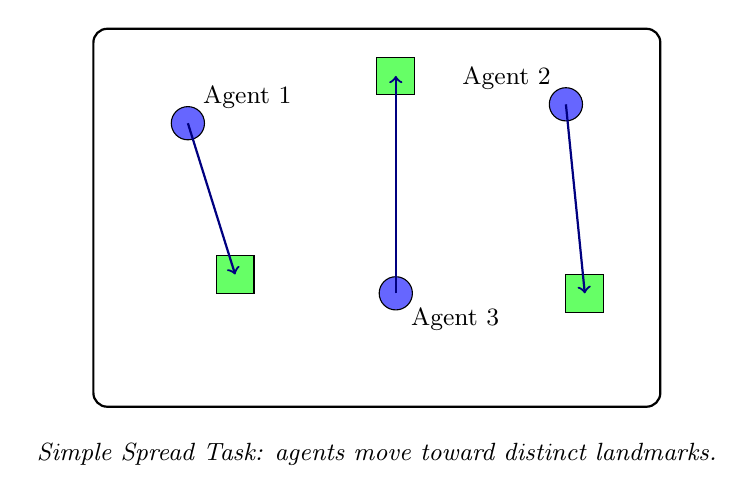
\begin{tikzpicture}[scale=1.2, every node/.style={font=\small}]
% Draw bounding box
\draw[thick, rounded corners=5pt] (0,0) rectangle (6,4);
% Agents (blue circles)
\coordinate (a1) at (1,3); \coordinate (a2) at (5,3.2); \coordinate (a3) at (3.2,1.2);
\filldraw[fill=blue!60] (a1) circle (5pt) node[above right=2pt] {Agent 1};
\filldraw[fill=blue!60] (a2) circle (5pt) node[above left=2pt] {Agent 2};
\filldraw[fill=blue!60] (a3) circle (5pt) node[below right=2pt] {Agent 3};
% Landmarks (green squares)
\coordinate (l1) at (1.5,1.4); \coordinate (l2) at (3.2,3.5); \coordinate (l3) at (5.2,1.2);
\filldraw[fill=green!60] (l1) ++(-0.2,-0.2) rectangle ++(0.4,0.4);
\filldraw[fill=green!60] (l2) ++(-0.2,-0.2) rectangle ++(0.4,0.4);
\filldraw[fill=green!60] (l3) ++(-0.2,-0.2) rectangle ++(0.4,0.4);
% Arrows from agents to landmarks
\draw[->, thick, blue!50!black] (a1) -- (l1); \draw[->, thick, blue!50!black] (a2) -- (l3); \draw[->, thick, blue!50!black] (a3) -- (l2);
% Label
\node at (3,-0.5) {\textit{Simple Spread Task: agents move toward distinct landmarks.}};
\end{tikzpicture}
\caption{Illustration of the \texttt{simple\_spread} task in MPE: agents (blue) must coordinate to cover all landmarks (green) while avoiding collisions.}
\label{fig:mpe_simple_spread}
\end{figure}


\subsubsection{StarCraft Multi-Agent Challenge (SMAC).}
For a more rigorous evaluation of large-scale tactical coordination, we use the \textbf{StarCraft Multi-Agent Challenge (SMAC)} as our primary benchmark. Built on top of the StarCraft II Learning Environment and commonly interfaced via the \textbf{PyMARL} framework, SMAC is the de-facto standard for benchmarking cooperative MARL algorithms. It is derived from StarCraft II, a popular and complex Real-Time Strategy (RTS) game, but focuses specifically on \textbf{micromanagement}: the tactical control of individual military units in combat, abstracting away the broader game's resource gathering and base building.

This focus makes SMAC an ideal testbed for decentralized control under severe partial observability. Each allied unit is controlled by an independent agent that receives observations only from its local field of view, simulating the "fog of war." Agents must learn to coordinate their movement, targeting, and use of abilities to defeat a team of enemy units controlled by the game's built-in AI.

The difficulty across SMAC scenarios varies significantly based on several factors:
\begin{itemize}
    \item \textbf{Scale}: The number of agents and enemies directly impacts the complexity of the joint action space.
    \item \textbf{Heterogeneity}: Scenarios with different unit types (e.g., Zealots, Stalkers, Marines) require agents to learn specialized roles based on their unique attributes (health, shields, attack range, speed). This poses a greater coordination challenge than homogeneous scenarios where all agents are identical.
    \item \textbf{Symmetry and Balance}: Scenarios can be symmetric (e.g., \texttt{3m} vs. 3 marines) or asymmetric (e.g., \texttt{5m\_vs\_6m}, where the allied team is outnumbered), testing the algorithm's robustness and ability to find non-trivial strategies.
\end{itemize}

\begin{table}[H]
    \centering
    \begin{tabular}{@{}llll@{}}
        \toprule
        \textbf{Scenario} & \textbf{Description} & \textbf{Difficulty} & \textbf{Type} \\ \midrule
        \texttt{3m} & 3 Marines vs. 3 Marines & Easy & Homogeneous, Symmetric \\
        \texttt{2s\_3z} & 2 Stalkers \& 3 Zealots & Medium & Heterogeneous, Symmetric \\
        \texttt{3s\_5z} & 3 Stalkers \& 5 Zealots & Hard & Heterogeneous, Symmetric \\
        \texttt{5m\_vs\_6m} & 5 Marines vs. 6 Marines & Hard & Homogeneous, Asymmetric \\ \bottomrule
    \end{tabular}
    \caption{Characteristics of selected SMAC benchmark scenarios.}    
    \label{tab:smac_scenarios}
\end{table}

Table~\ref{tab:smac_scenarios} summarizes a selection of scenarios that are often used for benchmarking, highlighting their distinct characteristics.

Furthermore, SMAC is highly \textbf{configurable}, which allows for controlled experiments and ablation studies. Researchers can modify key aspects of the environment, such as:
\begin{itemize}
    \item \textbf{State Information}: For Centralized Training, Decentralized Execution (CTDE) methods, the wrapper can provide a global state vector containing features like the health, position, and type of all ally and enemy units. This can be disabled to test fully decentralized training.
    \item \textbf{Reward Shaping}: The reward function can be a sparse signal (win/loss only) or a denser signal that includes damage dealt and received, facilitating learning.
\end{itemize}

The benchmark provides a range of challenging scenarios, such as \texttt{3m} (three marines vs. three marines), \texttt{2s\_3z} (two stalkers and three zealots), and \texttt{3s\_5z}, which are widely used to benchmark cooperative MARL methods under the CTDE paradigm.

\begin{figure}[H]
    \centering
    \includegraphics[width=\linewidth]{img/smac_maps.png}
    \caption{Example SMAC scenarios. Agents must coordinate to defeat enemy units using only local observations.}
    \label{fig:smac}
\end{figure}

\subsection{Focus on the SMAC Benchmark}
While MPE is valuable for validating fundamental concepts, the primary focus of our work is on the more demanding SMAC benchmark. This decision is motivated by several factors:
\begin{enumerate}
    \item \textbf{Scalability and Complexity}: SMAC provides a more significant challenge in terms of the number of agents, the complexity of their interactions, and the high-dimensionality of the problem, making it a better testbed for the robustness of advanced MARL algorithms.
    \item \textbf{Research Relevance}: As the most widely adopted benchmark for cooperative MARL, performance on SMAC allows for direct and meaningful comparison with a large body of state-of-the-art methods, including VDN, QMIX, and MAPPO.
    \item \textbf{Challenging Partial Observability}: The "fog of war" in SMAC is a much more difficult form of partial observability than the simple-radius vision in MPE, pushing algorithms to develop more sophisticated strategies for information gathering and decentralized execution.
\end{enumerate}
For these reasons, SMAC serves as the principal environment for validating our proposed methods.

\subsection{Development Infrastructure and Workflow}

To support large-scale experimentation, we established a robust and reproducible development pipeline. This section details the core infrastructure, monitoring tools, and the overall workflow that integrates them.

\subsubsection{Core Infrastructure and Version Control.}
Our primary computational resources consisted of several high-performance computing (HPC) nodes, accessed securely via SSH. To maintain consistency and enable collaboration, all code was managed using \textbf{Git and GitHub}. This provided a synchronized and version-controlled codebase across local development machines and remote servers, which is essential for reproducibility.

\subsubsection{Experiment Logging and Monitoring.}
For comprehensive experiment tracking, we integrated \textbf{Weights \& Biases (WandB)} into our training pipeline. As shown in Figures \ref{fig:wandb_logo} and \ref{fig:wandb_dashboard}, WandB serves as a centralized dashboard for real-time monitoring of key metrics, including:
\begin{itemize}
    \item \textbf{Performance metrics}: episode reward, win rate, and episode length.
    \item \textbf{Learning dynamics}: policy loss, Q-value estimates, and gradient norms.
    \item \textbf{Custom metrics}: agent-specific exploration rates and Q-value variance to analyze coordination.
\end{itemize}
This setup was invaluable for debugging, comparing model architectures, and generating clear visualizations. WandB's ability to group runs and execute hyperparameter sweeps also significantly streamlined our research process.

\begin{figure}[H]
    \centering
    \begin{minipage}{0.35\textwidth}
        \centering
        \includegraphics[width=0.8\linewidth]{img/logo/wandb.png}
        \caption{Weights \& Biases logo.}
        \label{fig:wandb_logo}
    \end{minipage}\hfill
    \begin{minipage}{0.6\textwidth}
        \centering
        \includegraphics[width=\linewidth]{img/wandb-demo.png}
        \caption{Example WandB dashboard.}
        \label{fig:wandb_dashboard}
    \end{minipage}
\end{figure}

\subsubsection{End-to-End Experimental Workflow.}
These components are integrated into a cohesive end-to-end experimental pipeline, illustrated in Figure~\ref{fig:workflow}. The process is a continuous cycle:
\begin{enumerate}
    \item \textbf{Local Development}: Model architectures and training scripts are written and tested locally.
    \item \textbf{Synchronization and Execution}: Using Git and SSH, the updated code is pushed to the remote HPC nodes. Training jobs are then launched using a custom script that wraps the \texttt{nohup} utility, ensuring they run reliably in the background.
    \item \textbf{Real-Time Tracking}: During training, all experimental data is streamed to WandB, allowing for live monitoring and analysis from a web-based dashboard.
    \item \textbf{Analysis and Iteration}: The insights gained from the WandB dashboards directly inform the next cycle of local development.
\end{enumerate}

\begin{figure}[H]
    \centering
    \includegraphics[width=0.9\linewidth]{img/workflow.png}
    \caption{Our high-level experimental workflow. The process is a continuous cycle: (1) Local development, (2) synchronization with remote machines for training, (3) real-time experiment tracking with WandB, and (4) analysis of results that informs the next development iteration.}
    \label{fig:workflow}
\end{figure}

\end{document}